\documentclass[sigconf]{acmart}

% Remove Fake Conference information
\settopmatter{printacmref=false} % Removes citation information below abstract
\renewcommand\footnotetextcopyrightpermission[1]{} % removes footnote with conference information in
\pagestyle{plain} % removes running headers
\acmDOI{}


\usepackage{pgfplots}
\usepackage{placeins}  % Required for \FloatBarrier
\usepackage{pgfplots}
\usepackage[table,xcdraw]{xcolor}
\usepackage{colortbl}
% Nice color sets, see see http://colorbrewer2.org/	
\usepgfplotslibrary{colorbrewer}
% initialize Set1-4 from colorbrewer (we're comparing 4 classes),
\pgfplotsset{compat = newest, cycle list/Set1-8} 
% Tikz is loaded automatically by pgfplots
\usetikzlibrary{pgfplots.statistics, pgfplots.colorbrewer} 
% provides \pgfplotstabletranspose
\usepackage{pgfplotstable}
\usepackage{filecontents}
\usepackage{booktabs}
\usepackage{listings} % Paquete para incluir código
\usepackage[utf8]{inputenc}
\usepackage[T1]{fontenc}





%%
%% \BibTeX command to typeset BibTeX logo in the docs
\AtBeginDocument{%
  \providecommand\BibTeX{{%
    \normalfont B\kern-0.5em{\scshape i\kern-0.25em b}\kern-0.8em\TeX}}}

%% Rights management information.  This information is sent to you
%% when you complete the rights form.  These commands have SAMPLE
%% values in them; it is your responsibility as an author to replace
%% the commands and values with those provided to you when you
%% complete the rights form.
\setcopyright{acmcopyright}
\copyrightyear{2023}
\acmYear{2023}
\acmDOI{}

% To remove fake conference data
\acmConference[]{}{}{, }


%%
%% Submission ID.
%% Use this when submitting an article to a sponsored event. You'll
%% receive a unique submission ID from the organizers
%% of the event, and this ID should be used as the parameter to this command.
%%\acmSubmissionID{123-A56-BU3}

%%
%% For managing citations, it is recommended to use bibliography
%% files in BibTeX format.
%%
%% You can then either use BibTeX with the ACM-Reference-Format style,
%% or BibLaTeX with the acmnumeric or acmauthoryear sytles, that include
%% support for advanced citation of software artefact from the
%% biblatex-software package, also separately available on CTAN.
%%
%% Look at the sample-*-biblatex.tex files for templates showcasing
%% the biblatex styles.
%%

%%
%% The majority of ACM publications use numbered citations and
%% references.  The command \citestyle{authoryear} switches to the
%% "author year" style.
%%
%% If you are preparing content for an event
%% sponsored by ACM SIGGRAPH, you must use the "author year" style of
%% citations and references.
%% Uncommenting
%% the next command will enable that style.
%%\citestyle{acmauthoryear}

%%
%% end of the preamble, start of the body of the document source.
\begin{document}

%%
%% The "title" command has an optional parameter,
%% allowing the author to define a "short title" to be used in page headers.
\title{Dependability Analysis - Apache commons-imaging library}

%%
%% The "author" command and its associated commands are used to define
%% the authors and their affiliations.
%% Of note is the shared affiliation of the first two authors, and the
%% "authornote" and "authornotemark" commands
%% used to denote shared contribution to the research.
\author{Martin Esteban Cardaci}
\authornote{All authors contributed equally to this research.}
\affiliation{%
  \institution{Università degli Studi di Salerno}
  \city{Fisciano}
  \state{Salerno}
  \country{Italy}
  \postcode{84084}
}
\email{m.cardaci@studenti.unisa.it}

\author{Johan Chicue Garcia}
\authornote{All authors contributed equally to this research.}
\affiliation{%
  \institution{Università degli Studi di Salerno}
  \city{Fisciano}
  \state{Salerno}
  \country{Italy}
  \postcode{84084}
}
\email{j.chicue@studenti.unisa.it}




%%
%% By default, the full list of authors will be used in the page
%% headers. Often, this list is too long, and will overlap
%% other information printed in the page headers. This command allows
%% the author to define a more concise list
%% of authors' names for this purpose.
\renewcommand{\shortauthors}{Martin E Cardaci, and Johan Chicue Garcia}

%%
%% The abstract is a short summary of the work to be presented in the
%% article.
\begin{abstract}
A comprehensive dependability analysis of the Apache Commons Imaging library, an open-source Java library for image processing, was conducted using a multifaceted approach. Tools such as SonarCloud, JaCoCo, PIT Mutation Testing, Randoop, and JMH were employed to assess code quality, automate testing, analyze vulnerabilities, and benchmark performance. The study identified test coverage gaps, improved the test suite, and revealed performance bottlenecks in compression algorithms, showcasing the impact of concurrency optimizations on throughput. Security vulnerabilities in dependencies were analyzed using OWASP Dependency Checker and SpotBugs, underscoring the need for robust dependency management and encapsulation. The analysis highlights the value of targeted testing and systematic quality assurance, offering actionable recommendations to enhance the library’s reliability and security.
\end{abstract}

%%
%% The code below is generated by the tool at http://dl.acm.org/ccs.cfm.
%% Please copy and paste the code instead of the example below.
%%
\begin{CCSXML}
<ccs2012>
   <concept>
       <concept_id>10011007.10011074.10011099.10011102.10011103</concept_id>
       <concept_desc>Software and its engineering~Software testing and debugging</concept_desc>
       <concept_significance>500</concept_significance>
    </concept>
    <concept>
       <concept_id>10011007.10011006.10011073</concept_id>
       <concept_desc>Software and its engineering~Software maintenance tools</concept_desc>
       <concept_significance>500</concept_significance>
   </concept>
   <concept>
       <concept_id>10011007.10011074.10011134.10003559</concept_id>
       <concept_desc>Software and its engineering~Open source model</concept_desc>
       <concept_significance>300</concept_significance>
   </concept>

 </ccs2012>
\end{CCSXML}

\ccsdesc[500]{Software and its engineering~Software testing and debugging}
\ccsdesc[500]{Software and its engineering~Software maintenance tools}
\ccsdesc[300]{Software and its engineering~Open source model}


%%
%% Keywords. The author(s) should pick words that accurately describe
%% the work being presented. Separate the keywords with commas.
\keywords{Apache Commons Imaging, Automated Test Case Generation, Bug Fixing, Code Coverage, Code Quality, CodeCov, SportBugs, JaCoCo, Java Microbenchmark Harness, JMH, Mutation Testing, OWASP Dependability Checker, PiTest, Software Analytics, Software Dependability, Software Engineering, Software Testing Tools, Software Vulnerabilities, SonarCloud, Randoop, Refactoring, Docker, Java}

%% \received{20 February 2007}
%% \received[revised]{12 March 2009}
%% \received[accepted]{5 June 2009}

%%
%% This command processes the author and affiliation and title
%% information and builds the first part of the formatted document.
\maketitle

\section{Introduction – Library target →  Apache Commons-Imaging}
Apache Commons Imaging \cite{apache-commons-imaging} is an open-source Java library designed for image processing, supporting a wide range of formats such as JPEG, PNG, GIF, BMP, and TIFF. With a focus on cross-platform compatibility and fostering collaboration, this library serves as an essential tool for Java developers requiring reliable and robust image processing capabilities.

A comprehensive analysis of software dependability within the Apache Commons Imaging project is conducted using a multifaceted approach. This process involves the application of software analytics, testing tools, and vulnerability assessment techniques to evaluate and enhance the project's dependability and code quality.

For the purpose of this project, a fork \cite{commons-imaging} of the original GitHub repository was created. 


\section{Project Management}
The allocation of tasks and responsibilities within the team was structured around two main approaches.
First, the focus was placed on coordinating the core aspects of the project, which included systematically setting up the environment required for executing tests, analyzing bug reports, classifying them, and identifying key areas to propose enhancements. Additional efforts were directed toward managing code optimization and generating updated results.
Second, attention was given to configuring the essential tools necessary to perform tests aimed at enhancing the reliability of the utilized library.
Team members collaborated closely across various tasks, including testing tools, coding, researching, and developing the final report, among other activities.

\section{Tools}

\subsection{Code review}
After analyzing the Commons-Imaging project on SonarCloud, the focus was placed on detecting, analyzing, and addressing all "high-severity" reliability issues to ensure the stability and security of the application. One identified issue pertained to a bad practice in Java \cite{Java_SE_Specifications} specifically related to accessing static members of subclasses from a parent class during static initialization.
It is essential to resolve this bad practice to prevent code fragility, hard-to-debug errors, and hidden issues. This is particularly critical in large or open-source projects, where other developers may unintentionally modify static members without recognizing their dependencies.
By addressing these issues early, the efficiency of the system is improved, risks are reduced, and the software becomes more reliable and sustainable over time.

\subsubsection{Analyzing SonarCloud Results}

Severities are now closely linked to the impacted aspects of software quality, with each affected area assigned a severity level. Among the five severity levels, issues were identified only at the high and low levels.

\textbf{High = 49}

These issues were addressed at their root through comprehensive refactoring, resulting in the elimination of all high-priority issues. Further details on the tasks undertaken can be found in Section 3.1.2.

\textbf{Low = 85}

Issues at this level have a minimal impact on the reliability of the software. Only three specific issues related to the statement "Remove this useless shift: Ints and longs should not be shifted by zero or more than their number of bits-1" were resolved. This selective approach was taken to prioritize addressing higher-impact problems, as outlined previously.

\begin{figure}[h!]
    \centering
    \includegraphics[width=1\linewidth]{reportSonarCloud.png}
    \caption{}
    \label{fig:enter-label}
\end{figure}

\subsubsection{Refactoring Proposal for Bug Fixes → AbstractFieldType.java}

The primary issues identified in the AbstractFieldType.java class were as follows:
    
    1. Direct Static Declarations:
The static fields, such as BYTE and ASCII, were directly initialized with specific instances (e.g., FieldTypeByte, FieldTypeAscii).

    2. Rigid and Explicit Dependency:
Each static field relied explicitly on the concrete field type classes (FieldTypeByte, FieldTypeAscii, etc.). This design introduced potential static initialization issues, particularly in scenarios involving cross-dependencies or complex declaration orders.

The changes implemented in the proposed refactoring were as follows:

• Use of a Helper Method:
A private static method, named createByteFieldTypeByName, was introduced to centralize the logic for creating field types. This method accepts a parameter (name) to identify the field type to be created and returns the corresponding instance based on the provided parameter.

\begin{lstlisting}[
    frame=single,
    breaklines,
    tabsize=4,
    linewidth=1\linewidth]{java}
private static AbstractFieldType createByteFieldTypeByName(String name) {
    if(Objects.equals(name, "BYTE")){
        return new FieldTypeByte(1, "Byte");
    }
}
\end{lstlisting}

• Deferred Initialization:
Static fields, such as BYTE and ASCII, are now initialized by invoking the createByteFieldTypeByName method. This approach ensures that field types are created dynamically, improving flexibility and mitigating potential initialization issues. 	

\begin{lstlisting}[
    frame=single,
    breaklines,
    tabsize=4,
    linewidth=1\linewidth]{java}
public static final AbstractFieldType BYTE = createByteFieldTypeByName("BYTE");
public static final AbstractFieldType ASCII= createByteFieldTypeByName("ASCII");
\end{lstlisting}

• Centralization of Initialization Logic:
Instead of explicitly declaring each field type, the centralized method now handles the initialization of instances. This reduces rigid dependencies, simplifies the management of the initialization order, and helps prevent accidental cycles. 

The main strategy focused on refactoring static initialization to reduce direct dependencies and centralize the logic in a single method. This was achieved through the following steps:

    1. Centralization of Object Creation:
The initialization logic was moved to the createByteFieldTypeByName method, effectively eliminating problematic explicit initializations.

    2. Deferred Initialization:
A method was employed to initialize the static fields, ensuring that each field is created independently. This approach mitigates issues related to the declaration order.

    3. Reduced Coupling:
The direct dependency between static fields and concrete classes was eliminated, enhancing the code's robustness and making it more adaptable to future changes or extensions.

The refactor addressed the following critical areas:

1. Centralization and ordering of static initialization.
    
2. Utility methods to encapsulate creation logic.
    
3. Reduction of circular dependencies and concurrency issues.
    
4. Cleaner, more modular, and maintainable code.

\hfill\\
\textit{These improvements help mitigate the risk of critical errors such as deadlocks and race conditions, while also making the code more comprehensible and easier to extend.}\cite{REF.Commit-088c26d}

\subsubsection{Implementation to Demonstrate the Usage of the Refactored Abstract Class}

To demonstrate the usage of the refactored class from the Apache Commons-Imaging library, a Java web project was created. The github repository can be found at \cite{websiteswd} This project includes a page that allows users to upload an image and view information about its TIFF fields.

For the implementation of this proof of concept (POC), a Java web project was built, configured, and deployed with a reference to the Apache Commons Imaging library and a Tomcat application server for deployment. The application runs using Docker.

The implementation offers a simple, user-friendly, and responsive web interface for uploading an image. The image is processed on the server side using Apache Commons Imaging, enabling the extraction of TIFF fields (metadata) and their types via the refactored class. The results are then displayed on a formatted web page.

The implementation interacts with the \textbf{AbstractFieldType} class through the \textbf{TiffField} object when processing image metadata within the servlet:

\begin{lstlisting}[
    frame=single,
    breaklines,
    tabsize=4,
    linewidth=1\linewidth]{java}
for (TiffField field : tiffImageMetadata.getAllFields()) {
    imageInfo.add(String.format("Field: %s, Type: %s, Value: %s",
            field.getTagName(), 
            field.getFieldType().getName(), //Here we use AbstractFieldType
            field.getValue()));
}
\end{lstlisting}

This occurs because:

1. When a TIFF image is read using Imaging.getMetadata(imageBytes), Commons Imaging internally parses the structure of the TIFF image.

2. For each TIFF field encountered, a TiffField object is created, which contains:

◦ The field value

◦ The field type (which is an instance of AbstractFieldType)

◦ Tag information

3. AbstractFieldType serves as the base class for all possible TIFF field types. For example, when a field is of type BYTE, FieldTypeByte, which extends AbstractFieldType, is used internally.


\begin{lstlisting}[
    frame=single,
    breaklines,
    tabsize=4,
    linewidth=1\linewidth]{java}
public static final AbstractFieldType BYTE = createByteFieldTypeByName("BYTE");
public static final AbstractFieldType ASCII = createByteFieldTypeByName("ASCII");
public static final AbstractFieldType SHORT = createByteFieldTypeByName("Short");
//etc...
\end{lstlisting}

When processing a TIFF field in the servlet, the following steps occur:

    1. field.getFieldType() returns a specific instance of AbstractFieldType for that field.
    
    2. getName() calls the getName() method of AbstractFieldType, which returns the type name (e.g., "Byte", "ASCII", etc.).
    
    3. The field value is obtained through field.getValue(), which internally uses the abstract methods of AbstractFieldType to correctly interpret the bytes based on the field type.
    
\vspace{0,5cm}
For example, if a TIFF field is of type BYTE:

1. field.getFieldType() will return the BYTE instance of AbstractFieldType.
    
2. .getName() will return "Byte".
    
3. The value will be interpreted as a byte according to the implementation of getValue() in FieldTypeByte.

This structure allows Commons Imaging to uniformly handle all possible TIFF field types, each with its own data interpretation logic, while sharing a common interface through AbstractFieldType.    

\vspace{0,5cm}
Below is the UML class diagram illustrating the following key points:

    1. \textbf{Class Hierarchy:}
    
        ◦ AbstractFieldType is the abstract base class.
        
        ◦ The abstract methods are marked with an asterisk (*).
        
        ◦ The diagram includes the main attributes and methods of each class.
        
    2. \textbf{Concrete Classes Inheriting from AbstractFieldType:}
    
        ◦ FieldTypeByte (for BYTE and SBYTE)
        
        ◦ FieldTypeAscii (for ASCII)
        
        ◦ FieldTypeShort (for SHORT and SSHORT)
        
        ◦ FieldTypeLong (for LONG and SLONG)
        
        ◦ FieldTypeRational (for RATIONAL and SRATIONAL)
        
    3. \textbf{Relationships Between Classes:}
    
        ◦ TiffField contains a reference to AbstractFieldType.
        
        ◦ TiffImageMetadata contains a collection of TiffField.
        
        ◦ ImageUploadServlet processes TiffImageMetadata.

    4. \textbf{Work Flow in the Web Application:}
    
        ◦ The servlet processes the image and retrieves the metadata.
        
        ◦ The metadata contains TIFF fields.
        
        ◦ Each TIFF field has a specific type that inherits from AbstractFieldType.
\hfill\\        
\textbf{Important notes about the diagram:}

    • Arrows with a solid line and white triangle represent inheritance.
    
    • Arrows with a dashed line represent usage or dependency.
    
    • Only the most relevant methods are shown in the diagram for clarity.
    
    • Some auxiliary classes and methods were omitted to maintain a clean and clear diagram.

\begin{figure}[h!]
    \centering
    \includegraphics[width=1\linewidth]{class diagram UML.png}
    \caption{UML Diagram}
    \label{fig:enter-label}
\end{figure}

The usage chain follows this sequence:

    1. \textbf{ImageUploadServlet} → Initiates the process.
    
    2. \textbf{Imaging.getMetadata()} → Creates an instance of JpegImageMetadata.
    
    3. \textbf{JpegImageMetadata} → Contains TiffImageMetadata (EXIF).
    
    4. \textbf{TiffImageMetadata} → Contains a collection of TiffField.
    
    5. \textbf{TiffField} → Uses AbstractFieldType to interpret its data.
\newpage

\subsubsection{Deployment of the Web Project Using Docker}

The deployment of the web project was carried out using Docker Desktop, with the aim of demonstrating the usage of the refactored class in a practical environment. A Docker image was created and made available on DockerHub for orchestration, ensuring accessibility and reproducibility of the deployment process.

\textbf{Dockerfile Configuration}

A Dockerfile was constructed to package the Java web application into a container. The Dockerfile included the following configuration:


\begin{lstlisting}[
    frame=single,
    breaklines,
    tabsize=4,
    linewidth=1\linewidth]{config}
FROM tomcat:9.0.80-jdk17
COPY target/mywebsite-1.0-SNAPSHOT.war /usr/local/tomcat/webapps/mywebsite.war
EXPOSE 8080
CMD ["catalina.sh", "run"]
\end{lstlisting}

\textit{This setup uses a Tomcat 9 base image with JDK 17, copies the built WAR file into the webapps directory, and exposes port 8080 for application access. The command catalina.sh run ensures the Tomcat server starts automatically when the container is run.}

\vspace{0,5cm}
\textbf{Deployment Process}

After building the web project, the following steps were executed:
    
    1. Stopped and removed any existing container with the same name to avoid conflicts:
    
docker stop contenedor-mywebsite

docker rm contenedor-mywebsite
    
    2. Built the Docker image for the project:

docker build -t mywebsite .

    3. Deployed the container, binding it to port 8080:
    
docker run -d -p 8080:8080 --name contenedor-mywebsite mywebsite
       
\textit{These steps ensured that the application was successfully deployed and running in a Docker container.}


\vspace{0,5cm}
\textbf{Publishing the Docker Image to DockerHub}

To enable further orchestration, the Docker image was tagged and pushed to DockerHub using the following commands:

    1. Tagged the image with the repository name and version:
       docker tag mywebsite:latest martincardaci/mywebsite:1.0.0

    2. Pushed the image to DockerHub:
       docker push martincardaci/mywebsite:1.0.0
    
    3. Verified the deployment by running the image directly from DockerHub:
       docker run -d -p 8080:8080 martincardaci/mywebsite:1.0.0

\textit{These steps made the image publicly available for reuse and testing.}

\vspace{0,5cm}
\textbf{Results and Validation}

The deployment process was validated through the following observations:

    1. Application Running in the Browser: The web application was accessible via http://localhost:8080/mywebsite, demonstrating the functionality of the deployed system.
    
    2. DockerHub Repository: The image was successfully uploaded and listed in the DockerHub repository martincardaci/mywebsite, confirming the correct execution of the push command.

    3. Container Status: The command docker ps displayed the running container, providing details such as container ID, image, and exposed port.

\textit{Screenshots of the application running in the browser, the DockerHub repository, and the docker ps output are included below to provide visual confirmation of the successful deployment.}

\begin{figure}[H]
    \centering
    \includegraphics[width=1\linewidth]{web1.png}
    \caption{}
    \label{fig:enter-label}
\end{figure}

\begin{figure}[H]
    \centering
    \includegraphics[width=1\linewidth]{web2.png}
    \caption{}
    \label{fig:enter-label}
\end{figure}

\begin{figure}[H]
    \centering
    \includegraphics[width=1\linewidth]{web3.png}
    \caption{}
    \label{fig:enter-label}
\end{figure}
\begin{figure}[H]
    \centering
    \includegraphics[width=1\linewidth]{web4.png}
    \caption{}
    \label{fig:enter-label}
\end{figure}
\begin{figure}[H]
    \centering
    \includegraphics[width=1\linewidth]{web5.png}
    \caption{}
    \label{fig:enter-label}
\end{figure}

\begin{figure}[H]
    \centering
    \includegraphics[width=1\linewidth]{dockerhub1.png}
    \caption{}
    \label{fig:enter-label}
\end{figure}
\begin{figure}[H]
    \centering
    \includegraphics[width=1\linewidth]{dockerhub2.png}
    \caption{}
    \label{fig:enter-label}
\end{figure}
\begin{figure}[H]
    \centering
    \includegraphics[width=1\linewidth]{dockerPS.png}
    \caption{}
    \label{fig:enter-label}
\end{figure}







\subsection{Software Testing Tools}

Effective testing is a cornerstone of software dependability, ensuring that code performs as intended under various conditions while minimizing the risk of defects. This report evaluates the coverage and robustness of the selected Java-based library using three complementary tools: JaCoCo\cite{jacoco} (Java Code Coverage) for code coverage base line analysis, PIT Mutation Testing \cite{pitest} for assessing test suite robustness, and Randoop\cite{randoop} for automated test generation. Each tool provides unique insights into the effectiveness of existing test cases and identifies areas for improvement, contributing to a comprehensive understanding of the library’s test coverage and dependability.


\subsubsection{JaCoCo - Java Code Coverage}
\hfill\\
JaCoCo is a tool used to measure the extent of code coverage achieved by existing test suites, providing baseline metrics to evaluate testing effectiveness. In this study, JaCoCo was integrated into the build process through Maven, with its plugin configured in the pom.xml file to enable automated instrumentation of the code during testing. Upon executing the tests, JaCoCo generated a detailed report that quantified coverage metrics at multiple levels.

\begin{figure}[h!]
    \centering
    \includegraphics[width=1\linewidth]{Coverage_Metrics.png}
    \caption{Coverage Metrics}
    \label{fig:enter-label}
\end{figure}

As seen on fig a.a, the analysis revealed an overall instruction coverage of 77.6\%, with 21,380 out of 95,452 instructions remaining untested. While this indicates a satisfactory level of coverage, there is considerable room for improvement. Branch coverage was reported at 64.3\%, with 2,567 out of 7,199 branches missed, exposing gaps in testing conditional logic. Additionally, 16,901 lines of code were covered, leaving 3,760 lines untested. Method and class coverage metrics were robust, with nearly all methods covered, missing only 15 methods, and achieving 100\% class coverage.

Coverage varied significantly at the package level. For example, the org.apache.commons.imaging.internal package exhibited instruction coverage as low as 28\% and branch coverage of 25\%, highlighting significant deficiencies. In contrast, moderately performing packages like org.apache.commons.imaging.formats.tiff achieved 57\% instruction coverage and 51\% branch coverage, underscoring the need for targeted testing in these areas.

The determination of whether coverage is “good” or “bad” depends on the context and specific project goals. This analysis focused on classes with less than 70\% instruction coverage, prioritizing them for further investigation through mutation testing with PIT and random test generation using Randoop. While the overall instruction coverage of 77.6\% is reasonable, the significant number of untested instructions underscores the need to address untested code paths systematically.

\subsubsection{PIT Mutation Testing (Pitest)}
\hfill\\
Based on the results of the JaCoCo analysis, packages with the lowest coverage were selected for mutation testing to evaluate the robustness of the test suite. Mutation testing introduces deliberate modifications (mutations) into the code to assess whether existing tests can detect these changes.

\begin{table}[h!]
\centering
\resizebox{\columnwidth}{!}{%
\begin{tabular}{|c|c|c|c|c|}
\hline
\textbf{Package} & \textbf{Instruction (\%)} & \textbf{Branch (\%)} & \textbf{Line (\%)} & \textbf{Method (\%)} \\ \hline
imaging.internal.*      & 28 & 25 & 69 & 60 \\ \hline
formats.psd.dataparsers & 33 & 66 & 50 & 66 \\ \hline
formats.tiff.*          & 57 & 51 & 72 & 66 \\ \hline
formats.jpeg            & 60 & 44 & 75 & 69 \\ \hline
formats.tiff.taginfos   & 67 & 50 & 64 & 67 \\ \hline
formats.bmp             & 72 & 61 & 72 & 66 \\ \hline
formats.pcx             & 66 & 61 & 61 & 61 \\ \hline
formats.psd             & 68 & 43 & 68 & 75 \\ \hline
formats.xpm             & 69 & 59 & 59 & 69 \\ \hline
\end{tabular}%
}
\caption{Classes with the Lowest Coverage Identified}
\label{tab:PITclasses}
\end{table}

For a subset of 18 classes seen on table \ref{tab:PITclasses}, PIT mutation testing achieved 60\% line coverage, with 775 out of 1,285 executable lines covered. Mutation coverage was reported at 57\%, with 986 out of 1,726 mutants killed. Test strength, defined as the ratio of killed mutants to covered mutations, was 76\%, indicating reasonably effective tests but with room for improvement.

At package level, significant variability was observed. The \textbf{\texttt{imagi\allowbreak ng.common}} package demonstrated high metrics, with 95\% line coverage and 84\% mutation coverage, indicating a well-tested module. In contrast, the \textbf{\texttt{formats.psd.dataparsers}} package showed only 11\% mutation coverage, highlighting weaknesses in its test suite. Similarly, the \textbf{\texttt{imaging.package}}, despite its importance, exhibited low line coverage of 35\% and mutation coverage of 23\%, emphasizing the need for more comprehensive tests.

\begin{table}[h!]
\centering
\resizebox{6cm}{!}{%
\begin{tabular}{|c|c|c|}
\hline
\textbf{Metric} & \textbf{Subset Classes} & \textbf{All Classes} \\ \hline
Number of Classes & 18 & 288 \\ \hline
Line Coverage - JaCoCo Report & 77.6\% & 77.6\% \\ \hline
Line Coverage - PiTEST Report & 60\% & 77\% \\ \hline
Mutation Coverage & 57\% & 55\% \\ \hline
Test Strength & 76\% & 69\% \\ \hline
\end{tabular}%
}
\caption{PIT Mutation Testing Results}
\label{tab:PITResults}
\end{table}

When analyzing all the classes within the library, the overall line coverage increased to 77.6\%, while mutation coverage slightly decreased to 55\%, as seen on table \ref{tab:PITResults}. Test strength was higher for the smaller subset (76\%) compared to the larger set (69\%). Notably, the \textbf{\texttt{commons.\allowbreak imaging}} package improved significantly in both line coverage (from 35\% to 68\%) and mutation coverage (from 23\% to 40\%) when analyzing the full set of classes. These results underscore the trade-offs between focused testing of smaller subsets and broader coverage of the entire codebase.

The findings indicate that large-scale testing offers a broad overview, whereas targeted subsets provide deeper insights and enhance test coverage effectiveness. Striking a balance between these approaches is crucial to optimize testing efficiency. Moving forward, efforts should focus on packages with lower mutation and line coverage to strengthen the overall robustness of the test suite. Additionally, exploring uncovered mutations can help identify potential edge cases that may require targeted testing.

\subsubsection{Random Automatic Test Generator (Randoop)}
\hfill\\
To address deficiencies in code coverage identified through JaCoCo and mutation testing, Randoop was employed as an automated test generation tool. While the existing test suite achieved high coverage metrics, gaps remained in certain underperforming packages. Randoop was introduced to generate additional tests aimed at addressing these gaps.

The introduction of Randoop resulted in localized improvements in coverage metrics. For example, instruction coverage in \textbf{\texttt{formats\allowbreak.png}} increased to 80\%, while \textbf{\texttt{formats.tiff.photometricinter \allowbreak preters}} achieved 94\%. Branch coverage improvements were also observed; for instance, the \textbf{\texttt{formats.jpeg.decoder}} package reached 91\% branch coverage, demonstrating Randoop's effectiveness in exercising untested code paths.

\begin{figure}[h!]
    \centering
    \includegraphics[width=1\linewidth]{Coverage_Metrics_Randoop.png}
    \caption{Coverage Metrics for Randoop}
    \label{fig:randoop}
\end{figure}


Despite these localized gains, the overall coverage metrics showed only modest improvements. Instruction coverage increased slightly from 77.6\% to 77.8\%, and branch coverage rose from 64.3\% to 64.6\%. These results reflect the high baseline coverage achieved by the existing test suite, which left limited opportunities for substantial global improvements. However, Randoop successfully enhanced coverage in weaker-performing packages. For instance, line coverage in org.apache.commons.imaging improved from 72\% to 73\%, and in \textbf{\texttt{formats.png}}, it increased from 75\% to 76\%.

Further analysis revealed that Randoop’s tests were balanced in some areas. For example, in \textbf{\texttt{formats.png}}, line coverage of 76\% aligned closely with mutation coverage of 72\%, indicating both enhanced test breadth and fault-detection capability. Conversely, in \textbf{\texttt{formats.icns}}, line coverage reached 82\%, significantly outpacing mutation coverage of 61\%, suggesting potential gaps in fault detection.

Certain packages, such as \textbf{\texttt{imaging.internal}}, remained consistently underperforming, with line coverage stagnating at 28\% and mutation coverage remaining low. These results highlight the need for additional test generation efforts focused on such areas.

\begin{figure}[h!]
    \centering
    \includegraphics[width=1\linewidth]{Coverage_Metrics_Comparison.png}
    \caption{Coverage Metrics Comparison}
    \label{fig:enter-label}
\end{figure}

Randoop proved effective in complementing existing testing approaches, particularly in improving coverage in underperforming packages. While its impact on global metrics was modest, it successfully uncovered untested scenarios and enhanced localized coverage. This underscores the importance of integrating automated test generation as a complementary strategy alongside manual and mutation-based testing to address specific weaknesses in the test suite. Future efforts should focus on consistently underperforming packages to maximize the potential of Randoop and similar tools


\subsection{Benchmarking with JMH: Performance Evaluation of Compression Test Classes}

Performance testing was conducted using the Java Microbenchmark Harness (JMH\cite{jmh}), a framework specifically designed for accurately measuring Java code performance at the micro-operation level. In this study, the performance of a test class for the compression and decompression of TIFF images was evaluated. These operations are computationally intensive due to the use of complex algorithms such as Deflate, LZW, and Packbits, making the class a "heavy" load for the system. The benchmarks compared two versions of the class: the original version (TiffRoundtripTestORIGINAL) and an optimized version (TiffRoundtripTest).

\textbf{Environment Configuration and Test Details}

The tests were conducted in a controlled environment on a multi-core processor machine with sufficient memory to ensure that the results were not influenced by hardware limitations. JMH was configured to perform 25 iterations per test, with adequate "warm-up" time to stabilize the Just-In-Time (JIT) compiler. The performance metric collected was throughput (operations per millisecond), chosen for its relevance in evaluating systems with repetitive high-demand operations like compression tests.
\newpage
\textbf{Benchmarking Results: Comparison of Versions}

The original version (TiffRoundtripTestORIGINAL) consistently showed low performance,
with a throughput of approximately \(10^{-4}\) ops/ms across all tests. In contrast, the optimized version (TiffRoundtripTest) demonstrated significant improvements, achieving throughput values ranging from \(10^{-3}\) to \(0.003\) ops/ms depending on the operation. The most notable performance was observed in the \texttt{processUncompressed} test, which achieved a throughput three times higher than other operations.
The most striking difference is that the optimized version not only increases overall performance but also reduces variability across different operations. This indicates specific optimizations aimed at improving resource management and processing efficiency.


\begin{figure}[h]
    \centering
    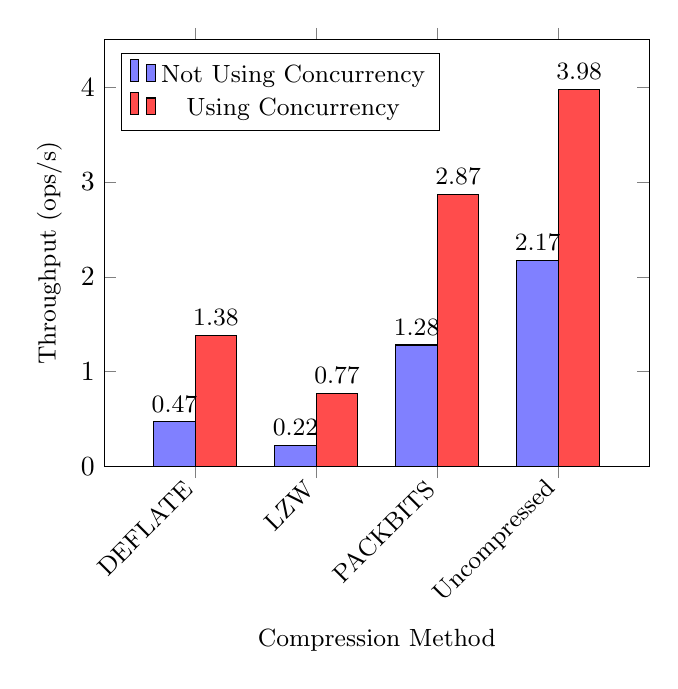
\begin{tikzpicture}
        \begin{axis}[
            ybar=0pt,
            bar width=15pt,
            width=8.5cm,
            height=7cm,
            enlarge x limits=0.25,
            ylabel={Throughput (ops/s)},
            xlabel={Compression Method},
            symbolic x coords={DEFLATE, LZW, PACKBITS, Uncompressed},
            xtick=data,
            ymin=0,
            ymax=4.5,
            xticklabel style={rotate=45, anchor=east, font=\small}, % Rotación de las etiquetas del eje x
            legend pos=north west,
            nodes near coords,
            every node near coord/.append style={font=\small},
            legend style={font=\small},
            ylabel style={font=\small},
            xlabel style={font=\small}
        ]
            % Original values (no concurrency)
            \addplot[fill=blue!50] coordinates {(DEFLATE, 0.47) (LZW, 0.22) (PACKBITS, 1.28) (Uncompressed, 2.17)};
            % Optimized values (with concurrency)
            \addplot[fill=red!70] coordinates {(DEFLATE, 1.38) (LZW, 0.77) (PACKBITS, 2.87) (Uncompressed, 3.98)};
            
            \legend{Not Using Concurrency, Using Concurrency}
        \end{axis}
    \end{tikzpicture}
    \caption{Throughput Comparison: Not Using vs. Using Concurrency}
    \label{fig:throughput_comparison}
\end{figure}

\textbf{Reasons for the Improvement in the Optimized Version}

Analysis revealed that the improvements in the optimized version were primarily achieved through a more efficient approach to parallelism and concurrency. While the original version relied on a sequential architecture, the optimized version introduced concurrent processes that leveraged the processor's multiple cores to divide compression and decompression tasks into independent threads. Additionally, memory management was optimized by reusing objects and buffers, significantly reducing allocation operations and garbage collection overhead.

\textbf{Conclusion}

The tests conducted with JMH highlight how enhancements in parallelism and algorithmic optimization can transform a resource-intensive test class into a more efficient and robust system. The optimized version not only increases throughput but also establishes a solid foundation for future improvements in applications that require handling large volumes of data efficiently. These tests emphasize the importance of using precise benchmarking tools to identify bottlenecks and validate the impact of implemented optimizations.







\subsection{Software Vulnerabilities}
Software vulnerabilities represent weaknesses or defects in a program that may be exploited by malicious actors to undermine the system's integrity, confidentiality, or availability. These vulnerabilities can manifest across various layers of software, ranging from conceptual design flaws to implementation errors. Addressing and remediating such vulnerabilities is imperative to maintain the software's security and reliability.

An OWASP Dependency Checker\cite{owasp-dependency-check} analysis was conducted to review the project's dependencies, providing critical insights into their contributions to overall system risk and potential security vulnerabilities.

SpotBugs\cite{spotbugs} complements OWASP Dependency-Check by examining source code for potential bugs and security vulnerabilities not directly associated with dependency management. Although SpotBugs is capable of identifying a wide spectrum of issues, this analysis was specifically confined to security-related warnings, as a thorough evaluation of code quality and general reliability had already been performed in section 3.1.

By integrating dependency analysis with source code inspection, this approach offers a comprehensive strategy to secure the software supply chain. The findings from this investigation establish a robust foundation for further exploration and mitigation efforts, aiming to enhance the software project's resilience and reliability.

\subsubsection{OWASP Dependability Checker}\hfill\\
The analysis identified the dependencies shown in the following table \ref{tab:OWASP}

\begin{figure}[h!]
    \centering
    \includegraphics[width=1\linewidth]{OWASP.PNG}
    \caption{OWASP Dependency Checker Report}
    \label{fig:OWASP_FIG}
\end{figure}

\begin{table}[h!]
\centering
\resizebox{\columnwidth}{!}{%
\begin{tabular}{|c|c|c|c|}
\hline
{\color[HTML]{000000} Dependency} & {\color[HTML]{000000} Highest Severity} & CVE Count & Confidence \\ \hline
{\color[HTML]{000000} jmh-core-1.37.jar} & NA & 0 & NA \\ \hline
{\color[HTML]{000000} jmh-generator-annprocess-1.37.jar} & NA & 0 & NA \\ \hline
{\color[HTML]{000000} jopt-simple-5.0.4.jar} & NA & 0 & NA \\ \hline
{\color[HTML]{000000} commons-io-2.18.0.jar} & MEDIUM & 1 & Highest \\ \hline
{\color[HTML]{000000} commons-math3-3.6.1.jar} & MEDIUM & 1 & Highest \\ \hline
{\color[HTML]{000000} junit-platform-console-standalone-1.9.2.jar} & CRITICAL & 1 & Low \\ \hline
\end{tabular}%
}
\caption{OWASP dependencies checker report summary}
\label{tab:OWASP}
\end{table}



\subsubsection{\textit{\textbf{Summary  of Findings}}}
\hfill\\

The analysis identified the following high-confidence dependencies:

\begin{itemize}
    \item \textbf{Commons IO 2.15.0}: Provides utility classes, stream implementations, file filters, file comparators, endian transformation classes, and additional functionality. 
    
    \item \textbf{Commons Math3 3.2}: Offers lightweight mathematics and statistics components addressing practical problems not directly supported by Java or commons-lang.
    
    \item \textbf{JMH Core 1.36}: Constitutes the JMH Core for Java Microbenchmarking Harness, referenced within the project scope of Apache Commons Imaging, version 1.0-SNAPSHOT.
    
    \item \textbf{JMH Generator Annprocess 1.36}: Represents the JMH Benchmark Generator based on Annotation Processors, also referenced in the project scope of Apache Commons Imaging, version 1.0-SNAPSHOT.
    
    \item \textbf{Jopt Simple 5.0.4}: A Java library for parsing command line options, referenced in the project scope of Apache Commons Imaging, version 1.36.

    \item \textbf{JUnit 5}: Provides a command-line interface for running JUnit 5 tests.
    
\end{itemize}

\hfill\\
{\textbf{Commons IO 2.15.0 and Commons Math3 3.2 Dependency Vulnerability}}
\hfill\\

The OWASP Dependency-Check report reveals that both dependencies are affected by \textbf{CVE-2021-37533}. Before version 3.9.0, the Apache Commons Net FTP client naively accepted the host address provided in the PASV response. This vulnerability could be exploited by a malicious server to redirect the client's connection to an unintended host. This redirection could potentially expose sensitive information about services running on the client's internal network. However, this attack vector requires the user to initially connect to the malicious server\cite{CVE_37}.

To mitigate this vulnerability, the default behavior was modified in version 3.9.0 to disregard such hosts by default, aligning with the behavior of tools like cURL. Additional details are documented in the Apache JIRA issue NET-711 \cite{Java_SE_Specifications}.

This CVE, which falls under the category of Common Vulnerabilities and Exposures, highlights a significant security concern within the Apache Commons Imaging project. It specifically pertains to a path traversal vulnerability that could be exploited to overwrite arbitrary files on the system when processing specially crafted image files. This issue underscores the importance of securing components used in image handling to prevent unauthorized system access or data modification.

\hfill\\
{\textbf{JUnit 5 Dependency Vulnerability}}
\hfill\\

The dependency junit-platform-console-standalone-1.9.2 is marked as critical in severity but exhibits low confidence in the OWASP Dependency-Check report. This dual classification warrants closer examination.

\begin{itemize}
    \item \textbf{Critical Severity}: JUnit is a widely adopted testing framework. Any vulnerabilities within this dependency could potentially allow attackers to exploit testing environments. In scenarios where testing and production systems overlap, attackers might modify test data or execute unauthorized actions. This risk justifies the critical severity classification. 

    \item \textbf{Low Confidence}: The low confidence level indicates that OWASP Dependency-Check did not find conclusive evidence to confirm the reported vulnerability. This suggests the possibility of a false positive. Best practices recommend manual verification of CVE entries for such cases.
\end{itemize}

\hfill\\
{\textbf{Examination of CVE-2022-31514}}
\hfill\\

The report references a single vulnerability, \textbf{CVE-2022-31514}, associated with the dependency. A manual review of the National Vulnerability Database (NVD) \cite{NVD} reveals that this CVE entry has been updated and is currently under reanalysis. This reanalysis could result in:
\begin{itemize}
    \item Adjustments to the CVE’s severity (e.g., modification of the CVSS score).
    \item Refinement of the affected software versions.
    \item Reclassification as either a non-vulnerability or a confirmed threat.
\end{itemize}

Due to its modified status, the CVE introduces ambiguity regarding the actual risk posed by this dependency. Consequently, it is essential to continuously monitor updates from the NVD and reassess the dependency’s impact as new information becomes available.

These findings serve as a basis for further investigation and remediation efforts to enhance the robustness of the project's software supply chain.




\subsubsection{SpotBugs}
\hfill\\
This section focuses on security-related warnings generated by SpotBugs during the static analysis of the library. The analysis identified four specific types of warnings within the "Malicious code vulnerability" category, as summarized in table \ref{tab:spotbugs}. Only medium priority warnings were found. Each warning type was examined, and its relevance and impact were evaluated. 

\begin{table*}[h!]
\centering
\resizebox{\textwidth}{!}{%
\begin{tabular}{|c|c|c|c|}
\hline
\textbf{Type of Warning} & \textbf{Problem classification} & \textbf{Number of Classes} & \textbf{Class Example} \\ \hline
\textbf{Field should be package protected} & MS\_PKGPROTECT & 1 & \textit{org.apache.commons.imaging.roundtrip.FullColorRoundtrip.images} \\ \hline
\textbf{Field should be both final and package protected} & MS\_FINAL\_PKGPROTECT & 3 & org.apache.commons.imaging.roundtrip.GrayscaleRountripTest.images \\ \hline
\textbf{May expose internal representation by returning reference to mutable object} & EI\_EXPOSE\_REP & 11 & org.apache.commons.imaging.formats.tiff.TiffField.getFieldType() \\ \hline
\textbf{May expose internal representation by incorporating reference to mutable object} & EI\_EXPOSE\_REP2 & 26 & org.apache.commons.imaging.formats.tiff.TiffField \\ \hline
\end{tabular}%
}
\caption{Summary Results for SpotBugs}
\label{tab:spotbugs}
\end{table*}

\hfill\\
{{\textbf{Field Should Be Package Protected}}
\hfill\\

The warning Field Should Be Package Protected highlights potential risks associated with mutable static fields that could be inadvertently or maliciously modified due to excessive visibility. To mitigate this, static analysis tools such as SpotBugs recommend reducing the visibility of such fields to package-protected.

In the case of the class \textbf{\texttt{roundtrip.FullColorRoundtrip}}, the warning is triggered for the field images. However, this warning is considered a false positive. The \textbf{\texttt{FullColorRoundtrip}} class is utilized exclusively within a testing context and is not part of the production codebase. The images field, while technically mutable, serves as controlled static test data and is accessed only within the scope of unit tests. Consequently, there is no practical risk of external access or unintentional modification. SpotBugs, as a static analysis tool, does not infer runtime context, leading to an unnecessary warning in this instance.
\newpage

{\textbf{Field Should Be Both Final and Package Protected}}
\hfill\\

This warning is raised when a mutable static field is neither declared final nor restricted in visibility. The recommended approach is to declare such fields as final and package-protected to ensure immutability and prevent unintended modifications.

The fields images in the classes \textbf{\texttt{roundtrip.GrayscaleRound\allowbreak tripTest}}, \textbf{\texttt{roundtrip.LimitedColorRoundtripTest}}, and \textbf{\texttt{round\allowbreak trip.BitmapRoundtripTest}} trigger this warning. These classes, similar to \textbf{\texttt{FullColorRoundtrip}}, are confined to unit test packages. The images fields in these classes act as static test data and are not exposed beyond their designated test scope. While the arrays are mutable, there is no practical risk of corruption due to the absence of external consumers and production usage.

Thus, the warnings for these classes arise from the inherent limitations of static analysis tools, which cannot distinguish between production code and test environments. The fields do not pose any substantive risk in this context.

\hfill\\
{\textbf{May Expose Internal Representation by Returning Reference to Mutable Object}}
\hfill\\

The warning May expose internal representation by returning a reference to a mutable object addresses concerns related to encapsulation. This warning is triggered when a class exposes mutable fields, such as arrays or objects, through public methods, thereby enabling unintended external modifications.
The severity of this warning is context-dependent. If the class is utilized internally or within a controlled environment, such as testing, the risk of unintended modification is minimal. In this analysis, several flagged cases emerged where this warning is either partially applicable or justified based on specific design considerations.

Notably, a significant number of flagged cases belong to the \textbf{\texttt{formats.tiff}} package. The design of classes such as \textbf{\texttt{TiffRaster\allowbreak DataFloat}} reflects a deliberate trade-off between memory efficiency and strict encapsulation. For instance, the methods \textbf{\texttt{getData()}} and \textbf{\texttt{getIntData()}} in \textbf{\texttt{TiffRasterDataFloat}} return direct references to internal arrays to optimize performance when handling large TIFF images. These arrays may contain over 100 million raster cells, and creating redundant copies of such data could exceed the memory capacity of a Java application.
While returning mutable references introduces risks related to data integrity, this decision prioritizes performance and resource utilization. The design choice is intentional and justified within the context of processing large-scale TIFF files. Thus, the warning, though valid in a strict sense, should be interpreted as an acceptable trade-off for optimized performance in this package.

Conversely, the warning is valid for classes where mutable objects are exposed without sufficient justification. For example, the class \textbf{\texttt{formats.jpeg.JpegImageMetadata}} exposes mutable fields via methods such as \textbf{\texttt{getExif()}} and \textbf{\texttt{getPhotoshop()}}. These methods return direct references to the fields \textbf{\texttt{exif}} and \textbf{\texttt{photoshop}}, respectively, thereby violating encapsulation principles. In such cases, external consumers of the class may inadvertently or maliciously alter the internal state. Consequently, the warning is applicable and highlights a genuine security and reliability concern.

\hfill\\
{\textbf{May Expose Internal Representation by Incorporating Reference to Mutable Object}}
\hfill\\

This related warning occurs when a class stores externally provided mutable objects without creating a defensive copy. Similar to the previous case, the severity of this warning depends on the context.

For instance, in the class \textbf{\texttt{formats.jpeg.JpegImageMetadata}}, the constructor stores mutable objects, such as \textbf{\texttt{JpegPhotoshopMeta\allowbreak data}} and \textbf{\texttt{TiffImageMetadata}}, directly into its internal fields. This design exposes the class to potential modifications by external consumers, which may lead to unintended side effects. Such warnings represent valid concerns and warrant corrective measures, such as defensive copying of mutable inputs.

The analysis of SpotBugs warnings revealed that a subset of the reported issues, particularly those within test-only classes, can be safely disregarded due to their restricted scope and controlled environment. Warnings associated with TIFF classes highlight intentional design choices aimed at balancing performance and memory efficiency when handling large data structures. These decisions, while introducing potential risks, are justified within the given context.

However, warnings related to JPEG metadata classes, which expose mutable objects externally, represent valid concerns and should be addressed to ensure proper encapsulation and maintain data integrity.
Static analysis tools, such as SpotBugs, offer significant value in identifying vulnerabilities but are limited by their inability to account for runtime contexts.  Consequently, a contextual review of each warning is essential to assess its relevance and impact accurately.
\newpage

\section{Conclusion}

This study underscores the importance of adopting holistic approaches to evaluate and enhance the quality, security, and performance of software projects. Future work should extend this analysis to additional modules of the library, explore advanced optimization techniques, and continue strengthening security by proactively mitigating vulnerabilities. The main findings highlight:
\hfill\\\hfill\\

1. Code quality and optimization:
High-priority issues were addressed through the refactoring of key components, resulting in improved modularity, reduced static dependencies, and optimized initialization processes. These enhancements strengthen the library's maintainability and scalability.

2. Test coverage: Tools such as JaCoCo, PIT Mutation Testing, and Randoop identified deficiencies in specific areas while demonstrating the effectiveness of automated testing in enhancing code robustness. Notably, Randoop uncovered previously untested scenarios, significantly increasing coverage in critical packages.

3. Performance: Benchmarks conducted with JMH revealed that concurrency management and memory handling optimizations significantly improved the performance of the TIFF image compression and decompression algorithms. These enhancements not only increased overall throughput but also reduced variability across operations.

4. Security: Evaluations using OWASP Dependency Checker and SpotBugs identified vulnerabilities in dependencies and potential encapsulation issues. While some warnings were deemed low-impact or context-specific, others underscored the need for better protection of sensitive data.


%% -> REFERENCES Section --> sample-base.bib has the cite references descriptions.
%% The next two lines define the bibliography style to be used, and
%% the bibliography file.

\bibliographystyle{ACM-Reference-Format}
\bibliography{sample-base}

%%
%% If your work has an appendix, this is the place to put it.
\appendix
\end{document}